\documentclass[a4paper]{book}

\usepackage{geometry}
% make full use of A4 papers
\geometry{margin=1.5cm, vmargin={0pt,1cm}}
\setlength{\topmargin}{-1cm}
\setlength{\paperheight}{29.7cm}
\setlength{\textheight}{25.1cm}

% auto adjust the marginals
\usepackage{marginfix}

\usepackage{amsfonts}
\usepackage{amsmath}
\usepackage{amssymb}
\usepackage{amsthm}
%\usepackage{CJKutf8}   % for Chinese characters
\usepackage{ctex}
\usepackage{enumerate}
\usepackage{graphicx}  % for figures
\usepackage{layout}
\usepackage{multicol}  % multiple columns to reduce number of pages
\usepackage{mathrsfs}  
\usepackage{fancyhdr}
\usepackage{subfigure}
\usepackage{tcolorbox}
\usepackage{tikz-cd}
\usepackage{listings}
\usepackage{xcolor} %代码高亮
\usepackage{braket}
%------------------
% common commands %
%------------------
% differentiation
\newcommand{\gen}[1]{\left\langle #1 \right\rangle}
\newcommand{\dif}{\mathrm{d}}
\newcommand{\difPx}[1]{\frac{\partial #1}{\partial x}}
\newcommand{\difPy}[1]{\frac{\partial #1}{\partial y}}
\newcommand{\Dim}{\mathrm{D}}
\newcommand{\avg}[1]{\left\langle #1 \right\rangle}
\newcommand{\sgn}{\mathrm{sgn}}
\newcommand{\Span}{\mathrm{span}}
\newcommand{\dom}{\mathrm{dom}}
\newcommand{\Arity}{\mathrm{arity}}
\newcommand{\Int}{\mathrm{Int}}
\newcommand{\Ext}{\mathrm{Ext}}
\newcommand{\Cl}{\mathrm{Cl}}
\newcommand{\Fr}{\mathrm{Fr}}
% group is generated by
\newcommand{\grb}[1]{\left\langle #1 \right\rangle}
% rank
\newcommand{\rank}{\mathrm{rank}}
\newcommand{\Iden}{\mathrm{Id}}

% this environment is for solutions of examples and exercises
\newenvironment{solution}%
{\noindent\textbf{Solution.}}%
{\qedhere}
% the following command is for disabling environments
%  so that their contents do not show up in the pdf.
\makeatletter
\newcommand{\voidenvironment}[1]{%
  \expandafter\providecommand\csname env@#1@save@env\endcsname{}%
  \expandafter\providecommand\csname env@#1@process\endcsname{}%
  \@ifundefined{#1}{}{\RenewEnviron{#1}{}}%
}
\makeatother

%---------------------------------------------
% commands specifically for complex analysis %
%---------------------------------------------
% complex conjugate
\newcommand{\ccg}[1]{\overline{#1}}
% the imaginary unit
\newcommand{\ii}{\mathbf{i}}
%\newcommand{\ii}{\boldsymbol{i}}
% the real part
\newcommand{\Rez}{\mathrm{Re}\,}
% the imaginary part
\newcommand{\Imz}{\mathrm{Im}\,}
% punctured complex plane
\newcommand{\pcp}{\mathbb{C}^{\bullet}}
% the principle branch of the logarithm
\newcommand{\Log}{\mathrm{Log}}
% the principle value of a nonzero complex number
\newcommand{\Arg}{\mathrm{Arg}}
\newcommand{\Null}{\mathrm{null}}
\newcommand{\Range}{\mathrm{range}}
\newcommand{\Ker}{\mathrm{ker}}
\newcommand{\Iso}{\mathrm{Iso}}
\newcommand{\Aut}{\mathrm{Aut}}
\newcommand{\ord}{\mathrm{ord}}
\newcommand{\Res}{\mathrm{Res}}
%\newcommand{\GL2R}{\mathrm{GL}(2,\mathbb{R})}
\newcommand{\GL}{\mathrm{GL}}
\newcommand{\SL}{\mathrm{SL}}
\newcommand{\Dist}[2]{\left|{#1}-{#2}\right|}

\newcommand\tbbint{{-\mkern -16mu\int}}
\newcommand\tbint{{\mathchar '26\mkern -14mu\int}}
\newcommand\dbbint{{-\mkern -19mu\int}}
\newcommand\dbint{{\mathchar '26\mkern -18mu\int}}
\newcommand\bint{
	{\mathchoice{\dbint}{\tbint}{\tbint}{\tbint}}
}
\newcommand\bbint{
	{\mathchoice{\dbbint}{\tbbint}{\tbbint}{\tbbint}}
}





%----------------------------------------
% theorem and theorem-like environments %
%----------------------------------------
\numberwithin{equation}{chapter}
\theoremstyle{definition}

\newtheorem{thm}{Theorem}[chapter]
\newtheorem{axm}[thm]{Axiom}
\newtheorem{alg}[thm]{Algorithm}
\newtheorem{asm}[thm]{Assumption}
\newtheorem{defn}[thm]{Definition}
\newtheorem{prop}[thm]{Proposition}
\newtheorem{rul}[thm]{Rule}
\newtheorem{coro}[thm]{Corollary}
\newtheorem{lem}[thm]{Lemma}
\newtheorem{exm}{Example}[chapter]
\newtheorem{rem}{Remark}[chapter]
\newtheorem{exc}[exm]{Exercise}
\newtheorem{frm}[thm]{Formula}
\newtheorem{ntn}{Notation}

% for complying with the convention in the textbook
\newtheorem{rmk}[thm]{Remark}


%\lstset{
%	backgroundcolor=\color{red!50!green!50!blue!50},%代码块背景色为浅灰色
%	rulesepcolor= \color{gray}, %代码块边框颜色
%	breaklines=true,  %代码过长则换行
%	numbers=left, %行号在左侧显示
%	numberstyle= \small,%行号字体
%	keywordstyle= \color{blue},%关键字颜色
%	commentstyle=\color{gray}, %注释颜色
%	frame=shadowbox%用方框框住代码块
%}
\lstset{
	columns=fixed,       
	numbers=left,                                        % 在左侧显示行号
	numberstyle=\tiny\color{gray},                       % 设定行号格式
	frame=none,                                          % 不显示背景边框
	backgroundcolor=\color[RGB]{245,245,244},            % 设定背景颜色
	keywordstyle=\color[RGB]{40,40,255},                 % 设定关键字颜色
	numberstyle=\footnotesize\color{darkgray},           
	commentstyle=\it\color[RGB]{0,96,96},                % 设置代码注释的格式
	stringstyle=\rmfamily\slshape\color[RGB]{128,0,0},   % 设置字符串格式
	showstringspaces=false,                              % 不显示字符串中的空格
	language=c++,                                        % 设置语言
}

%----------------------
% the end of preamble %
%----------------------

\begin{document}
\pagestyle{empty}
\pagenumbering{roman}

%\tableofcontents
%\clearpage

%\pagestyle{fancy}
%\fancyhead{}
%\lhead{Qinghai Zhang}
%\chead{Notes on Algebraic Topology}
%\rhead{Fall 2018}


\setcounter{chapter}{0}
\pagenumbering{arabic}
% \setcounter{page}{0}

% --------------------------------------------------------
% uncomment the following to remove these environments 
%  to generate handouts for students.
% --------------------------------------------------------
% \begingroup
% \voidenvironment{rem}%
% \voidenvironment{proof}%
% \voidenvironment{solution}%


% each chapter is factored into a separate file.

\chapter{算法设计文档}

\section{数学概念的包装}

以下的dim都是模板参数维数.


\subsection{方程求解器, class equationsolver<dim>}
这个类是方程求解的接口,
\subsubsection{属性:}
\begin{itemize}
	\item 离散点的数量. int n[dim];
	\item 离散点各个维度上的距离.  Real h[dim];
	\item 存储每个网格点上目标函数v的值.  Real* value;
	\item 存储每个网格点上右端函数f的值.  Real* fvalue;
	\item 存储每个网格点上离散方程的残差值. Real* rvalue;
	\item 将高维坐标转化为在一维存储数组坐标的操作类指针 coordinate* pcoord
	\item 各个环节采用不同的方式的记录值,如松弛迭代时取用Jacobi迭代或者Gauss-Seidel迭代. 
	 boundary\_type btype = Diri;
	restrict\_operator restrictop = full;
	interpolat\_operator interpolatop = linear;
	cycle\_type ctype = V\_cycle;
	stop\_criteria stopcondi = maxstep;
	relax\_type rtype = GaussSeidel;
\end{itemize}

\subsubsection{操作:}
\begin{itemize}
	\item 初始化,必须输入网格数量n,间距h和边界条件和右端项在每个网格上的值fvalue.初始值和边界v是可选项(默认为0).   equationsolver(n ,h, fvalue, value).
	\item 输出存储的近似值value和残差rvalue.  pair<Real*,Real*> getresult() const;
\end{itemize}

\subsubsection{虚操作:需要在子类中重新定义}
\begin{itemize}
	\item 选取可选项.  bool chooseoption(name, type);
	\item 更新残差.    void updatervalue();
	\item 限制算子.    equationsolver* Restrict();
	\item 插值算子.    eqautionsolver* Interpolate();
	\item 松弛算子.    void Relax();
	\item 求解函数.    void solver(v, stopcondition);
	
\end{itemize}

\subsection{泊松方程求解器,class possionsolver<dim> : public equationsolver<dim>}
泊松方程的求解器,继承求解器的接口.

没有额外的固有属性
\subsubsection{操作:}
\begin{itemize}
	\item 实现equationsolver中的所有虚操作.
	\item 各种松弛算子.     void RB\_GaussSeidel\_Relax();
	void Relax(Rv);
	void Jacobirelax(v,f,result);
	
	\item 分别实现全权重限制算子和插入限制算子.  void Fullrestrict(v, result);
	\item 插值算子. equationsolver* Linearinterpolate();
	
\end{itemize}

\subsection{多重网格循环方式, class cycle<dim>}
这是个操作类,不含有属性. class Vcycle,class FMGcycle 分别从中继承实现接口

\subsubsection{虚操作:}
\begin{itemize}
	\item 对求解器psolver进行一次循环运算,循环参数为v. 
	void operator(psolver, v); 
\end{itemize}

\section{UML类图}

\begin{figure}
	\centering
	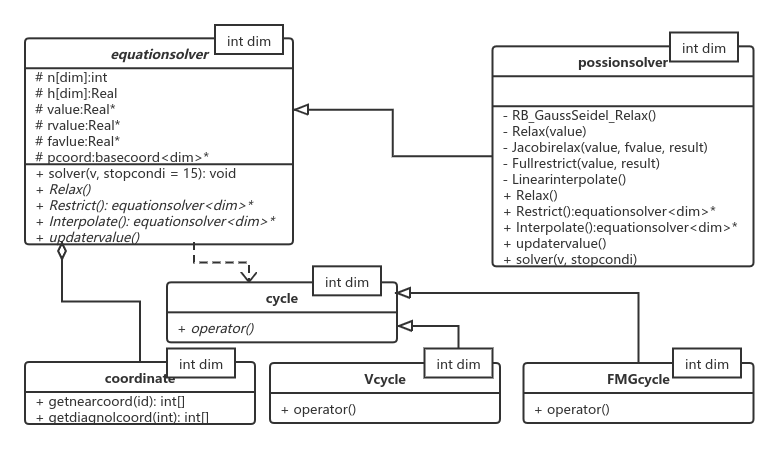
\includegraphics[width=18cm,height=14cm]{multigrid.png}
	\caption{多重网格程序UML类图}
\end{figure}


\end{document}


%%% Local Variables: 
%%% mode: latex
%%% TeX-master: t
%%% End: 

% LocalWords:  FPN underflows denormalized FPNs matlab eps IEEE iff
% LocalWords:  cardinality significand quadratically bijection unary
%  LocalWords:  contractive bijective postcondition invertible arity
%  LocalWords:  subspaces surjective injective monomials additivity
%  LocalWords:  nullary Abelian abelian finitary eigenvectors adjoint
%  LocalWords:  eigenvector nullspace Hermitian unitarily multiset
%  LocalWords:  nonsingular nonconstant homomorphism homomorphisms
%  LocalWords:  isomorphically indeterminates subfield isomorphism
%  LocalWords:  nondefective diagonalizable contrapositive cofactor
%  LocalWords:  submatrix nilpotent positivity orthonormal extremum
%  LocalWords:  Jacobian nonsquare semidefinite nonnegative RHS LLS
%  LocalWords:  roundoff closedness
